
% This overabundance of ribosomes
% provides different challenges on the ability of the cell to maintain steady-state
% growth under limiting nutrient conditions, and in Supplemental
% Section XX we consider this slow growth regime further.

% While this dependence between cell size and ribosomal abundance is apparent
% across moderate to fast growth rates, it is worth noting that

% This scaling behavior is likely to change at slow growth rates (below $\lambda
% \approx 0.5\,\text{hr}^{-1}$). Here, the number of ribosomes $R$ no longer
% reflects the cell's protein synthesis capacity, so far taken to be $r_t \ R$.
% Instead, cells reduce the number of actively translating ribosomes through the
% additional regulatory control of the small-molecule alarmone, guanosine
% pentaphosphate [(p)ppGpp] \citep{dai2016} [more citations].

\subsection{[Header for final section??]}

The relationship between cell size, actively translating ribosomes, and growth
rate, suggest that cells tune their size and ribosomal abundance as a way to
match their biosynthetic capacity to the available nutrient conditions. As one
illustration of this, disruption of the major glucose uptake system PTS through
the deletion of \textit{ptsG} doesn't just simply limit carbon uptake and
growth, which is reduced about two-fold. Rather, cells accommodate this
perturbation by also reducing their ribosomal fraction about two-fold
\citep{dai2016}; matching the expected decrease in growth rate governed by
\EQ{translation_limit_growth_rate} for this change in ribosomal fraction. In
this final section we consider a minimal model of growth rate control. We use it
to quantitatively show how changes in ribosomal content and total proteomic mass
will allow cells to maximize their growth rate according to the available
nutrient conditions.

To react to changes in nutrient conditions, bacteria rely on secondary-messenger
molecules like (p)ppGpp, which cause global changes in transcriptional and
translational activity.  In \textit{E. coli}, amino acid starvation causes the
accumulation of deacylated tRNAs at the ribosome's A-site and this leads to a
strong activation of (p)ppGpp synthesis activity by RelA \citep{hauryliuk2015}.
The dramatic decrease in active ribosomal fraction that is now apparent for
growth rates below about 0.5 hr$^{-1}$ ($f_a \approx$ 0.5 at a growth rate of
about 0.3 hr$^{-1}$, \cite{dai2016}) shows that (p)ppGpp also coordinates growth
in poor nutrient conditions. Furthermore, (p)ppGpp can inhibit DNA replication
initiation by mediating a change in transcriptional activity and the
supercoiling state of the origin of replication \citep{kraemer2019}. These
observations all raise the possibility that it through (p)ppGpp that cells
mediate the growth-rate dependent changes in $\langle$\# ori$\rangle$, cell size
and ribosomal abundance \citep{zhu2019, Buke2020}. Indeed, recent work in a
(p)ppGpp null strain found that cells exhibited a high ratio of $\langle$\#
ori$\rangle$ to $\langle$\# ter$\rangle$ and cell size that was more consistent
with a fast growth state where (p)ppGpp levels are normally low
\citep{fernandezcoll2020}.

To better understand how cells are able to maximize their growth rate under
different extents of nutrient limitation, we proceed by assuming that the rate
of elongation $r_t$ depends only on the availability of amino acids (and,
therefore, also amino-acyl tRNAs). It is at the level of amino acid synthesis
and availability that we will assume cells adjust their ribosomal abundance and
cell size (\FIG{translation_model}(A)). Other molecular players required for translation like elongation
factors and GTP are considered in sufficient abundance, which appear to be valid
assumptions given our analysis of the proteomic data and energy production thus
far.


\subsubsection{A Minimal Model of Nutrient-Limited Growth}

For simplicity, we proceed by considering amino acids as a single species, with a cellular
concentration $[AA]_{\text{eff}}$. The rate of elongation $r_t$ will depend on
how quickly ribosomes can match codons with their correct amino-acyl tRNA, as
well as the remaining steps required for peptide elongation. We therefore
consider that elongation will depend on two course-grained timescales, 1) the
time to find and bind each correct amino-acyl tRNA, and 2) the remaining steps
in peptide elongation that will not depend on the amino acid availability. The
time to translate each codon is given by the inverse of the elongation rate
$r_t$, which can be written as,

\begin{equation}
\frac{1}{r_t} = \frac{1}{k_{on} B [AA]_{\text{eff}}} + \frac{1}{r_{t}^{\text{max}}}.
\end{equation}
Here we have assumed that the rate of binding by amino-acyl tRNA $k_{on}$ is
proportional to $[AA]_{\text{eff}}$ by a constant $B$. The second term on the
right-hand side reflects our assumption that other steps in peptide elongation
are not rate-limiting, with a maximum elongation rate $r_{t}^{\text{max}}$ of
about 17 aa per second \cite{dai2016}. This can be rearranged more succinctly in
terms of an effective binding constant $K_d = r_{t}^{\text{max}}/ (k_{on} \ B)$,
with the elongation rate now given by,

\begin{equation}
r_t = \frac{r_{t}^{\text{max}}}{1 + K_d/[AA]_{\text{eff}}}.
\label{eq:rt_kd_simple}
\end{equation}

During steady-state
growth the amino acid concentration is constant ($d[AA]_{\text{eff}}/dt$=0). $[AA]_{\text{eff}}$
will relate to the
rate of amino acid synthesis (or import, for rich media)
$r_{aa}$ and consumption $r_t R f_a$ by,

\begin{equation}
\int_{0}^{\tau} \frac{d[AA]_{\text{eff}}}{dt} dt =  \int_{0}^{\tau} ([r_{aa}] - [r_t R f_a]) dt,
\end{equation}
where the time from 0 to $tau$ is a single cell doubling, and the square
brackets indicate of concentration per time. Solving this, we find that

\begin{equation}
[AA]_{\text{eff}} =  ([r_{aa}] - [r_t R f_a]) \tau.
\end{equation}
Alternatively, for an average cell size of $V$,  $[r_{aa}] = r_{aa}/(V N_A)$
and $[r_t R f_a] = (r_t R \ f_a)/(V N_A)$, where $N_A$ is Avogadro's
number. Since $\tau = ln(2)/\lambda$, which is also related to the parameters
$r_t R f_a$ and $N_{aa}$ through \EQ{mass_balance}, we
can also rewrite this as,

\begin{equation}
[AA]_{\text{eff}} = \frac{ln(2) N_{aa}}{V N_A} \left(\frac{r_{aa}}{r_t R f_a} - 1 \right) .
\label{eq:aa_final}
\end{equation}

By plugging in \EQ{aa_final} into \EQ{rt_kd_simple}, which also depends on $r_t$, we
can solve for $r_t$ explicitly. Its solution are the roots of a quadratic equation,
with the positive given by,

\begin{equation}
r_t = \frac{\sqrt{c^2 + 4 c k r_{t}^{\text{max}} - 2 c r_{t}^{\text{max}} + (r_{t}^{\text{max}})^2} - c - r_{t}^{\text{max}}}{2 \ (k-1)}.
\label{eq:rt_final}
\end{equation}
Here, $c = r_{aa}/(R f_a)$ and $k = N_A V K_d / N_{aa}$. In the final two
subsections we use this model to explore how the cell's metabolic capacity
($r_{aa}$) constrains the maximum growth rate, and then explain an apparent role
of for (p)ppGpp in mitigating translational activity at slow growth, where the
number of ribosomes is in excess.

\subsubsection{Optimal Growth Rate, Ribosomal Content, and Cell Size Depend on Nutrient
Availability and Metabolic Capacity.}

The way we will explore this model is to constrain the set of parameters based
on the growth-rate dependent proteomic changes in the available data under
nutrient limitation;  namely, we will restrict the values of $R$, $N_{aa}$, and
$V$ to those associated with the growth conditions in \cite{schmidt2016}. We
will then consider how changes in the nutrient conditions, through the parameter
$r_{aa}$, influence the maximum growth rate. In \FIG{translation_model}(B) we
plot the elongation rate $r_t$ for a high and low value of $r_{aa}$, reflective
of poor and rich nutrient conditions, respectively as a function of cellular
ribosome concentration [NB: need to state values used - maybe rationalize choice
of values based on the data]. Here we find that for high values of $r_{aa}$,
cells will be able to support protein synthesis and maintain a high rate of
elongation. However, for poor nutrient conditions (low $r_{aa}$), a high
abundance of ribosomes causes a dramatic decrease in $r_t$. In this regime, we
see that a reduction of actively translating ribosomes, through a decrease in
the parameter $f_a$, allow cells to maintain a high rate of elongation even
under more pronounced limits of nutrient limitation. By decreasing $f_a$,
through direct inhibition of available ribosomes, cells are able to maintain
homeostasis and keep $[AA]_{\text{eff}}$ relatively high (considered further in
Supplemental Section XX).

In \FIG{translation_model}(C) we show that for a particular cell state (i.e.
specific value of $R$, $N_{aa}$, and $V$), there will be a maximal growth rate
that depends on the capacity of the cell to provide amino acids to ribosomes.
Specifically, we see that the maximum growth rate $\lambda$ increases with
increasing $r_{aa}$, and corresponds to a cell with higher ribosomal fraction.
Importantly, however, there is an optimum  set of $R$, $N_{aa}$, and $V$ that
are strictly dependent on the value of $r_{aa}$. Increasing the ribosomal
concentration beyond the cell's metabolic capacity has the adverse consequence
of depleting the supply of amino acids and a concomitant decrease in the
elongation rate $r_t$ (\FIG{translation_model}(B)).


\begin{figure*}
    \begin{fullwidth}
    \centering{
        % 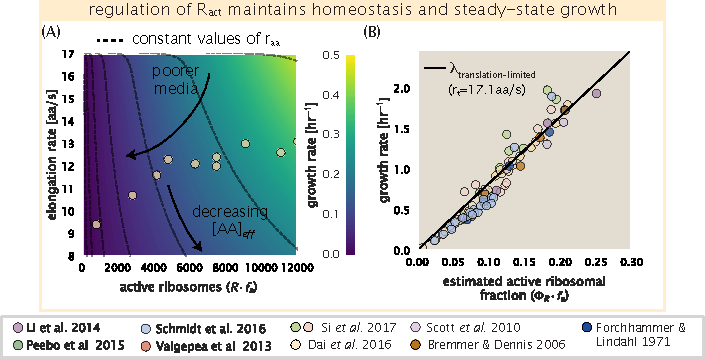
\includegraphics{main_figs/fig8_ribosome_growth_limit_ecoli_b_2.pdf}
        \caption{
        (A)
        (B)}
        \label{fig:translation_model}
    }
    \end{fullwidth}
\end{figure*}

%
%
% \subsubsection{\textit{E. coli} Maintains Growth in Poor Nutrient Conditions by a
% Reduction of Translation Activity.}
%
% In the slowest growth condition considered in the proteomic data, cells were
% grown in a chemostat ($\lambda$ = 0.12 hr$^{-1}$), and were found to have a ribosomal
% mass fraction of $\Phi_R \approx 0.06$ and of order 10$^4$ ribosomes per cell.
% In this absence of any additional regulation, we would predict a very low elongation rate of $r_t = X aa/s$.
%
% In contrast, wild-type \textit{E. coli} maintain a relatively high
% elongation rate even in stationary phase ($\approx$ 8 AA/s, \citep{dai2016,
% dai2018}).
%
% Careful
%
%
% In \FIG{}(B), we see that in the poorest nutrient conditions
% [NB: start by highlighting the dilemma when cells have excess ribosomes].
%
% How do cells regulate protein synthesis when amino acids become limiting,
% meaning that consumption exceeds the rate of synthesis? In the slowest  growth
% conditions, we find a minimum ribosomal mass fraction of $\Phi_R \approx 0.06$
% and  of order 10$^4$ ribosomes per cell.  Without the additional regulatory
% control noted above, there would be a point where  this imbalance would occur if
% all ribosomes were actively translating  (\FIG{translation_ecoli_partB}).
%
% Such a
% scenario would prevent continuous growth, and indeed for (p)ppGpp null strains,
% cells only grow in minimal media if additional amino acid supplements are
% present. In contrast, wild-type \textit{E. coli} maintain a relatively high
% elongation rate even in stationary phase ($\approx$ 8 AA/s, \citep{dai2016,
% dai2018}).
%
% To better understand how regulation of ribosomes influence growth rate at
% slow growth, we consider a coarse-grained model that relates elongation
% rate to a limiting supply of amino acids, which for simplicity we treat as a
% single, effective rate-limiting species $[AA]_{eff}$. Under such a scenario, the elongation
% rate $r_t$ can be described as depending on the maximum elongation rate ($r_t^{max}
% \approx$ 17.1 AA/s, \citep{dai2016, dai2018}), an effective binding constant
% $K_D$ between the pool of amino acids and their amino-acyl tRNAs, and the limiting
% amino acid concentration $[AA]_{eff}$,
%
% \begin{equation}
% r_t = r_t^{max} \cdot \frac{1}{1 + K_D / [AA]_{eff}}.
% \label{eq:rate_Kd}
% \end{equation}
% For cells growing in minimal medium supplemented with glucose, the amino acid
% concentration is of order 100 mM (BNID: 110093, \citep{milo2010, bennett2009}).
% To estimate  $K_D$, we note that for a growth rate of about 0.6 hr$^{-1}$
% \cite{dai2016} measured an elongation rate of about 12.5 AA$\cdot$s$^{-1}$,
% yielding $K_D \approx 40$ mM. The maintenance of this amino acid pool
% $[AA]_{eff}$ will depend on the difference between the synthesis/supply rate of
% amino acids $r_{AA}$ and consumption by ribosomes $r_t \times R \times f_a$,
% where we use $f_a$ to account for the possible reduction of actively translating
% ribosomes (see Supplemental Appendix XX for further details on this model).
%
% In \FIG{translation_ecoli_partB}(B), we show the relationship between the growth
% rate and elongation rate as a function of the number of actively translating
% ribosomes. Here, growth rate is now determined by the active ribosomal fraction via
% \begin{equation}
% \lambda_\text{translation-limited} \approx \frac{r_t}{L_R}  \Phi_R f_a.
% \label{eq:translation_limit_growth_rate_2}
% \end{equation}
% If we consider constant values of amino acid synthesis rate $r_{AA}$ (dashed
% lines) to reflect the available parameter space for a specific growth condition,
% the fastest growth rates result from  maximization of the fraction of actively translating
% ribosomes. When we consider the experimental measurements from \cite{dai2018}
% (yellow circles), reflecting growth in different nutrient conditions, we see
% that although $R \times f_a$ is reduced in poorer nutrient conditions, it is
% reduced in a manner such that $[AA]_{eff}$ is relatively constant. Given our estimate
% $K_D \approx$ 40 mM,  we would only expect a decrease from 100 mM to about 35 mM
% in the slowest growth conditions. While experimental data is scarce, data from
% \cite{bennett2009} show that amino acid
% concentrations only decrease to about 60 mM for cells grown in minimal media
% supplemented with acetate ($\lambda \approx$  0.3 hr$^{-1}$ in our proteomic data)
% \citep{bennett2009}, qualitatively consistent with our expectations. One
% explanation for the experimental data is that the active fraction of the
% ribosome pool is regulated in order to maintain a sufficient supply of amino acids for
% growth. Any further increase in $R \times f_a$ at constant $r_{AA}$ would
% otherwise be associated with an additional drop in cellular amino acid
% concentration.
%
% \begin{figure*}
%     \begin{fullwidth}
%     \centering{
%         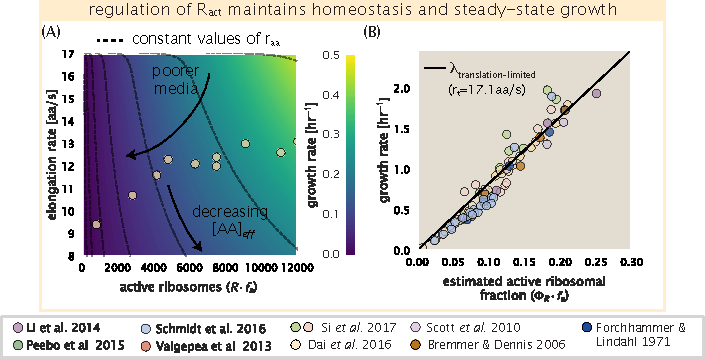
\includegraphics{main_figs/fig8_ribosome_growth_limit_ecoli_b_2.pdf}
%         \caption{\textbf{\textit{E. coli} must regulate ribosomal activity in
%         limiting nutrient conditions. }
%         (A) Translation elongation rate is plotted
%         as a function of the number of actively translating ribosomes $R
%         f_a$. Dashed lines correspond to a range of amino acid synthesis rates
%         $r_{aa}$, from 10$^3$ to 10$^6$. Growth rates are calculated according
%         to Equation 1, assuming a constant ribosomal fraction of 8 percent. See
%         appendix XX for additional details.}
%         \label{fig:translation_ecoli_partB}
%     }
%     \end{fullwidth}
% \end{figure*}
%

%
% [important point is that as resources become limiting, cells are able to tune and minimize
% the entire cell mass - which enables them to grow faster]
%
% [Discuss implications of findings so far. All other components being tuned (mostly) in the required proportions; and also that the achievable growth rate is ultimately set by ribosomes. ]
%
% [The apparent constraint that cells MUST get larger in order to grow faster places a particular constrain on why a cell would vary its ribosomal fraction in the first place.]
%
% [Also present the evidence from literature that there is a prominent role for aa/nutrient sensing that appears to mediate X, Y, and Z. ]
%
% [Then go on to propose the way to understand what’s going on with our model.
%     - I think maybe it’s easiest to understand it is we start by considering the balance that must be maintained between metabolic activity and ribosomal activity.
%     - Then write down a model that relates how elongation rate will relate to this.]
%
%
%

% [Figure idea: PART (A) Maybe we can consider that r_t*R sets the maximum rate of growth; but you also need to feed that engine and build the house to fit them.]
%
% [ When I get into slow growth regime; consider that IF R scales with <#ori>, ribosomes will have increasingly longer wait times for protein synthesis. Which is bad.
%     - By also decreasing the fraction of actively translating ribosomes, cells can grow faster is also super important. ]
%
%
%
%
